

The EUTelescope package \cite{Corrin2009} provides software tools for offline analysis and reconstruction of telescope test beam data. 
EUTelescope is embedded into the ILCSoft framework which provides the basic building blocks for offline analysis such as a data model (Linear Collider I/O, \emph{LCIO}),
 a geometry description language (\emph{GEAR}) and the central event processor (\emph{Marlin}) \cite{EUDET-2008-48}. 
EUTelescope comes with its own job submission framework \emph{jobsub} that allows to run analysis jobs locally or to submit them to larger computing clusters such as NAF.

Marlin allows the modular composition of analysis chains for various applications since every task is implemented as an independent \emph{processor} that is called by Marlin. 
The processors expose a set of parameters to the user which can be configured and loaded at runtime via so-called \emph{steering files} in XML format.
This way the Marlin/Processor architecture gives a lot of flexibility to the end user. 

EUTelescope provides several processors for Marlin implementing algorithms necessary for a full track reconstruction and data analysis of beam test experiments. 
Figure~\ref{fig:offline:strategy} shows the analysis strategy of the framework starting from the recorded detector response to the final aligned particle tracks. 
%An overview of the processor range provided by EUTelescope is given in \cite{EUDET-2007-20}.
For low-energy beams such as the DESY-II and ELSA testbeam facilities multiple scattering is the dominating source of track resolution uncertainties. 
Therefore EUTelescope provides advanced algorithms such as General Broken Lines (GBL) \cite{Kleinwort-2012} for tracking which accounts for scattering in all material present in the beam. 
In addition, precise software alignment can be performed using the Millipede-II algorithm \cite{Blobel-2006}.

Support for tracking in presence of magnetic fields and a more fine-grained detector geometry description interface using ROOT::TGeo are currently under development.

\begin{figure}[tbp]
	\center
	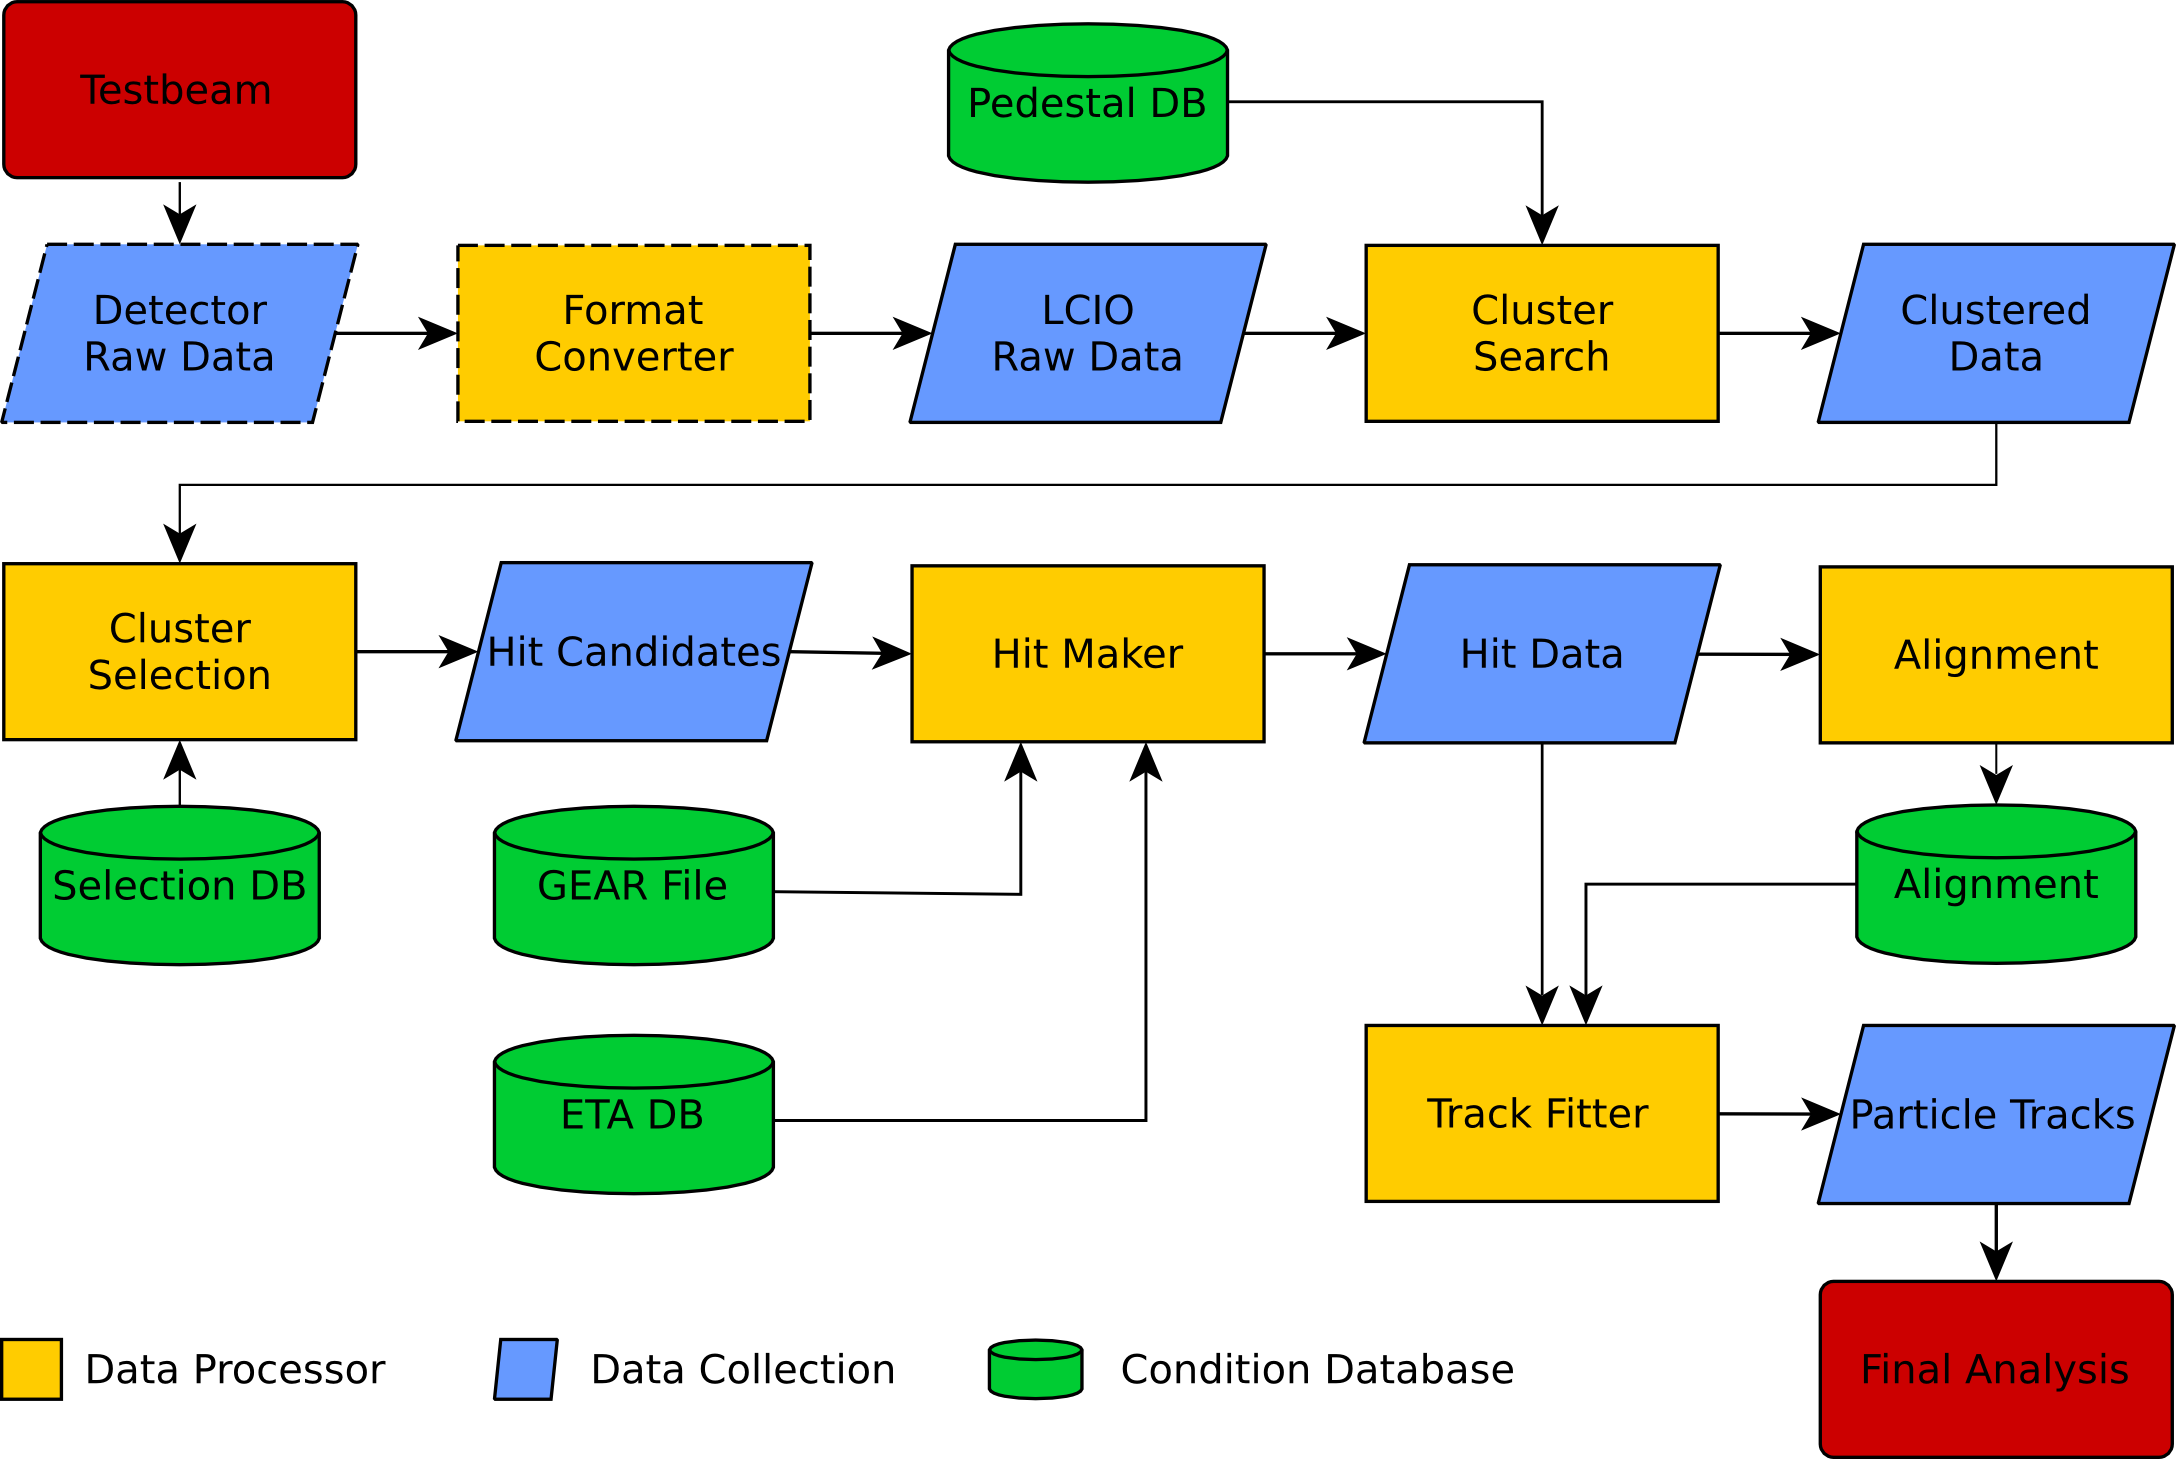
\includegraphics[width=.9\textwidth]{figures/eutel-strategy.png}
	\caption[The EUTelescope data analysis strategy]{Schematic of the overall telescope data reconstruction and analysis strategy of the EUTelescope framework. 
	EUTelescope provides processors for all steps except for the ones with dashed outline; these have to be implemented by the user.}
	\label{fig:offline:strategy}
\end{figure}

